\begin{aufgabe}{Codes}{4}
Gegeben sei der \jmark[Code]{mrk:Code} $C = \{ 00110, 11010, 10001, 01101 \}$.
\begin{enumerate}[label=\alph*)]
    \item Ist $C$ \jmark[linear]{mrk:LinearerCode}?
    \item Berechnen Sie die \jmark[Hammingdistanz]{mrk:Hammingabstand} $d(01101, 11010)$.
    \item Über einen verrauschten Kanal wurden die Wörter $01010$ sowie $10100$ empfangen.
    Dekodieren Sie, sofern möglich, mittels des \jmark[Maximum-Likelihood]{mrk:MaxLikely} Verfahrens die empfangenen Wörter.
    \item Bestimmen Sie das maximale $t$, sodass $C$ $t$-Fehler korrigierend ist.
\end{enumerate}
\Splitter
\vspace{-1\baselineskip}
\begin{enumerate}[label=\alph*)]\narrowitems
    \item Offensichtlich handelt es sich bei $C$ nicht um einen linearen Code. So gilt zum Beispiel: \(00110 \oplus 11010 = 11100 \not\in C\)
    \item Es gilt: \(d(01101, 11010) = 4\) (da: \(01101 \oplus 11010 = 10111 \text{ und } w(10111) = 4\))
    \item Wir betrachten die Fälle getrennt:
    \begin{itemize}[label=--]\narrowitems
        \item $01010$: Formal berechnen wir \(d(a, c)~\forall c \in C\): \begin{multicols}{2}
            \begin{itemize}[label=]\narrowitems
                \item \(d(01010, 00110) = 2\)
                \item \(d(01010, 11010) = 1\)
                \item \(d(01010, 10001) = 4\)
                \item \(d(01010, 01101) = 3\)
            \end{itemize}
        \end{multicols}
        Da hier eindeutig ein Wort zugeordnet werden kann sagen wir: Nach dem Maximum-Likelihood Verfahren evaluiert $01010$ zu $11010$
        \item $10100$: Wieder berechnen wir für jedes Codewort die Hammingdistanz:
        \begin{multicols}{2}
            \begin{itemize}[label=]\narrowitems
                \item \(d(10100, 00110) = 2\)
                \item \(d(10100, 11010) = 3\)
                \item \(d(10100, 10001) = 2\)
                \item \(d(10100, 01101) = 3\)
            \end{itemize}
        \end{multicols}
        Da sich hier kein Codwort eindeutig zuordnen lässt ist eine Dekodierung nicht möglich!
    \end{itemize}
    \item Wir kennen die Formel \(t = \left\lfloor \frac{d-1}{2}\right\rfloor \) müssen nun also nur noch den Minimalabstand von $C$ ($d(C)$) berechnen: 
    \begin{multicols}{3}
        \begin{itemize}[label=]\narrowitems
            \item \(d(00110, 11010) = 3\)
            \item \(d(00110, 10001) = 4\)
            \item \(d(00110, 01101) = 3\)
            \item \(d(11010, 10001) = 3\)
            \item \(d(11010, 01101) = 4\)
            \item \(d(10001, 01101) = 3\)
        \end{itemize}
    \end{multicols}
    Mit $d(C) = 3$ erhalten wir: \(t = \left\lfloor \frac{3-1}{2}\right\rfloor = 1\)
\end{enumerate}
\end{aufgabe}
\newpage
\begin{aufgabe}{Linearer Code}{2}
    Gegeben sei der folgende Code $C=\{11100, 10010, 01010\}$.
    \begin{enumerate}[label=\alph*)]
        \item Ergänzen Sie $C$ zu einem linearen Code $D$.
        \item Was ist der höchste Wert für $k$, sodass $D$ $k$-systematisch ist?
    \end{enumerate}
\Splitter
Im Folgenden wurde kramphaft versucht den Überblick zu erhalten:\smallskip
\begin{enumerate}[label=\alph*)]
    \item Hierzu verxoren wir alle Codwörter miteinander, bis kein neues Codewort mehr entsteht (hier überschwänglich ausgeführt). Wichtig sei angemekrt, da die Codwörter auch mit sich selbst verxort werden liegt $00000$ immer in $D$. Wir erhalten weiter:
    \begin{multicols}{2}
        \begin{itemize}[label=]\narrowitems
            \item \(11100 \oplus 10010 = 01110\)
            \item \(11100 \oplus 01010 = 10110\)
            \item \(10010 \oplus 01010 = 11000\)
            \item \(11100 \oplus 01110 = \textcolor{gray}{10010}\)
            \item \(11100 \oplus 10110 = \textcolor{gray}{01010}\)
            \item \(11100 \oplus 11000 = 00100\)
            \item \(11100 \oplus 00100 = \textcolor{gray}{11000}\)
            \item \(10010 \oplus 01110 = \textcolor{gray}{11100}\)
            \item \(10010 \oplus 10110 = \textcolor{gray}{00100}\)
            \item \(10010 \oplus 00100 = \textcolor{gray}{10110}\)
            \item \(01010 \oplus 11000 = \textcolor{gray}{10010}\)
        \end{itemize}
    \end{multicols}
    Damit erhalten wir den Code:\begin{centered}
        $D = \{11100,10010, 01010, 01110,10110,11000,00100,00000\}$
    \end{centered}
    \item Relativ leicht sehen wir, dass $D$ in den Stellen $2-4$ (also $k = 3$) systematisch ist:     
    \begin{multicols}{3}
        \begin{itemize}[label=]\narrowitems
            \item \(000 \Rightarrow 0\mathbf{000}0\)
            \item \(001 \Rightarrow 1\mathbf{001}0\)
            \item \(010 \Rightarrow 0\mathbf{010}0\)
            \item \(011 \Rightarrow 1\mathbf{011}0\)
            \item \(100 \Rightarrow 1\mathbf{100}0\)
            \item \(101 \Rightarrow 0\mathbf{101}0\)
            \item \(110 \Rightarrow 1\mathbf{110}0\)
            \item \(111 \Rightarrow 0\mathbf{111}0\)
        \end{itemize}
    \end{multicols}
\end{enumerate}
\end{aufgabe}\newpage
\begin{aufgabe}{Allgemeine Hammingschranke}{3}
Sei also $C$ ein $t$-Fehler-korrigierender Code der Länge $n$ mit
Alphabetgröße $\sigma$. Leiten Sie die allgemeine Hammingschranke für $C$ in
Abhängigkeit von $\sigma$ her. Benutzen Sie dazu (analog zu binären Codes) den
Hammingabstand als Anzahl der Stellen, an denen sich zwei Vektoren $x,y \in \Sigma^n$ unterscheiden.
\Splitter
Wie bereits in der Vorlesung erwähnt können wir uns die Codewörter eines Codes als Punkte in einem $\sigma$-Dimensionalem Körper vorstellen. Für binäre Codes entspricht dies einer Ebene. Bleiben wir zur Anschaulichkeit erstmal bei binären Codes und konstruieren uns nun Kreise um jedes Codewort mit maximaler Größe, so sodass sich keiner der Kreise mit einem anderen überschneidet:
\begin{wrapfigure}{l}{0.275\textwidth}
    \centering\vspace{-7pt}
    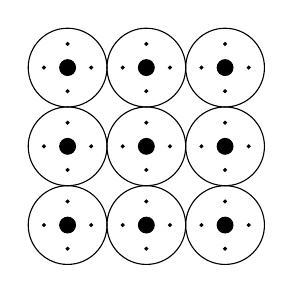
\begin{tikzpicture}
        \foreach \x in {1,...,3} {
            \foreach \y in {1,...,3}{
                \filldraw[black] (\x,\y) circle (0.1);
                \draw (\x,\y) circle (0.5);
                \foreach \sx/\sy in {0.3/0,-0.3/0,0/0.3,0/-0.3} {
                    \filldraw (\x+\sx,\y+\sy) circle (0.5pt);
                }
            }
        }
    \end{tikzpicture}
\end{wrapfigure}
Dies entspricht exakt der Definition eines \(t\)-Perfekten Codes. Im Zweidimensionalen bedeutet dies, dass alle Kreise den Radius \(t\) besitzen. Im 3-Dimensionalen entspricht diese Struktur einer Kugel und ab dem 4-Dimensionalen verabschiedet sich unsere Vorstellungskraft auch wenn die allgemeine Definition dieselbe bleibt: $$ B_t(c) \das \{x \in \Sigma^n \mid d(x,c) \leq t\}$$
In Worten: Die \say{Kugel} um $c \in C$ enthält alle Codewörter die zu $c$ einen Hammingabstand $\leq t$ besitzen. Bei einem perfekten binären Code wissen wir, dass die Kugel genau $|B_t(c)|$ Elemente enthalten kann: $$|B_t(c)| = \sum\limits_{e=0}^t\binom{n}{e}$$
Wobei \(n\) nach wie vor die Länge der Codewörter ist. Dies rührt aus folgender eigenschaft: Für $l$ Fehlstellungen ($d(x,c) = l$) gibt es \emph{$l$ aus $n$} mögliche Kombinationen wie diese im Codewort auftreten können (Eigenschaft Binomialkoeffizient). Haben wir einen Binärcode so gibt es nur $2$ Fälle, für die $1$ Ziffer verschieden sein kann: $1 - 0$ oder eben $0 - 1$. Haben wir aber nun einen Code über ein Alphabet mit $\sigma = 3$, so haben wir einige Stellungen mehr: $0 - 2$, $1 - 2$, \ldots\newline
Insgesamt finden wir genau $(\sigma -1)^l$ solcher zusätzlicher Varianten. Somit ergibt sich allgemein für die Kardinalität von $B_t(c)$: $$|B_t(c)| = \sum\limits_{e=0}^t(\sigma-1)^e \binom{n}{e}$$
Ein Code mit $|C|$ Wörtern besitzt zudem genau $|C|$ solcher Kugeln. Wir schreiben also: $$|\Sigma^n| \geq |C|\cdot |B_t(c)|$$
Das $\geq$ anstelle des $=$ steht hierbei, da wir ja nur bei einem perfekten Code von Gleichheit sprechen und es sich hierbei auch um die obere Schranke handelt (siehe Kugelgrafik). Mit $|\Sigma^n| = \sigma^n$ können wir nun noch nach $|C|$ umformen und erhalten somit unsere allgemeine Hammingschranke: 
$$|C| \leq \frac{\sigma^n}{\sum_{e=0}^t(\sigma-1)^e \binom{n}{e}}$$
\end{aufgabe}

\begin{aufgabe}{Perfektion}{3}
\vspace{-1\baselineskip}
\begin{enumerate}[label=\alph*)]\narrowitems
\item Gegeben sei ein binärer \([23,12,7]\)-Code. Ist dieser Code perfekt?
        Begründen Sie Ihre Antwort.
\item Ein binärer Blockcode \(\mathcal{C}\) der Länge \(n=5\) kann bis zu \(2\)
        Fehler korrigieren. Wie viele Codewörter hat \(\mathcal{C}\) höchstens?
        Geben Sie einen konkreten Code mit diesen Eigenschaften an.
\item Zeigen Sie, dass es keinen 1-perfekten binären Blockcode der Länge 13 gibt.
\end{enumerate}
\Splitter
\vspace{-1\baselineskip}
\begin{enumerate}[label=\alph*)]\narrowitems
    \item Für einen \(t\)-Perfekten Code muss gelten: \\
          \(|C| = 2^n \Big/ \left(\binom{n}{0} + \binom{n}{1} + \ldots + \binom{n}{t}\right)\) 
          Für \(t\) erhalten wir gemäß der Formel: \(t = \lfloor \frac{d-1}{2} \rfloor = \lfloor \frac{7-1}{2}\rfloor = 3\). Setzen wir nun unsere Werte in die Formel ein erhalten wir (da Binär gilt: \(|C| = 2^k\)): \\
          \(|C| = 2^{12} \overset{!}{=} 2^{23} \Big/ \left(\binom{23}{0} + \binom{23}{1} + \binom{23}{2} + \binom{23}{3}\right) = 4096 = 2^{12}\) \ding{51}. Es handelt sich also dabei um einen (\(3\)-)perfekten Code!
    \item Wählen wir für \(t = \lfloor \frac{d-1}{2} \rfloor = 2\) den Minimalabstand \(d\) minimal ergibt sich \(d=5\) und wir sehen offensichtlich, dass damit \({\cal C}\) nur 2 Codewörter haben kann, nämlich: \({\cal C} = \{00000,11111\}\).(Die Aufgabe wurde so interpretiert, dass ein Code der Länge 5 gesucht wird, welcher \(2\)-Fehler korrigierend ist und nicht einfach \(2^5\) als die maximale Anzahl möglicher binärer Blockcodes mit der Länge 5)
    \item Wir nehmen uns dazu wieder die Formel:  \\
    \(|C| = 2^n \Big/ \left(\binom{n}{0} + \binom{n}{1} + \ldots + \binom{n}{t}\right)\) \\
    Wir wählen gemäß den Informationen \(n=13\). Es ergibt sich (mit logisch \(n \geq k \in \N\)): \\
    \(|C| = 2^k \overset{?}{=} 2^{13} \Big/ \left(\binom{13}{0} + \binom{13}{1}\right) = \frac{2^{13}}{14} = 585.14 \ldots\). Offensichtlich ist die Gleichheit für kein \(k \in \N\) erfüllt \(\Rightarrow\) Es gibt keinen \(1\)-perfekten Blockcode der Länge 13. 
\end{enumerate}
\end{aufgabe}
\clearpage
\begin{aufgabe}{Paritätscode}{4}
Gegeben sei ein linearer Binärcode \(C\) der Länge \(n\). Wir hängen an jedes
Wort in \(C\) ein Paritätsbit an und erhalten so den Code \(C'\):
\[
    C' \das \quad\smashoperator{\bigcup_{\substack{(c_1,...,c_n)\in
    C}}}\quad \{(c_1,\dots,c_n,\,c_1\!\oplus \ldots \oplus c_n)\} \,.
\]
\begin{enumerate}[label=\alph*)]
\narrowitems
    \item Zeigen Sie, dass \(C'\) ebenfalls ein linearer Code ist.
    \item Sei nun \(C\) ein 2-perfekter Code.
        Leiten Sie den Minimalabstand von \(C'\) her.
\end{enumerate}
\Splitter
\begin{enumerate}[label=\alph*)]\narrowitems
    \item Seien im folgenden, o.B.d.A, \(a,b,c,d \in {\cal C}\) und \(w(a) \equiv w(b) \equiv 0 \mod 2\), \(w(c) \equiv w(d) \equiv 1 \mod 2\). Aufgrund der Linearität von \({\cal C}\) genügt es das Paritätsbit für folgende Fälle zu betrachten: \(a \oplus b, b \oplus c\) (da: \(c \oplus b\) analog) und \(c \oplus d\). Es ergibt sich:\\
    \(p(a\oplus b) = 0 = p(a) \oplus p(b), p(b \oplus c) = 1 = p(b) \oplus p(c), p(c \oplus d) = 0 = p(c) \oplus p(d)\). Somit gilt offensichtlich die Linearität, auch wenn \({\cal C}\) zum Beispiel keine \(c,d\) enthalten würde, da die Linearität für alle Fälle zutrifft und somit lediglich weniger Fälle betrachtet werden müssten. Damit ist gezeigt, dass es sich bei \({\cal C}'\) ebenfalls um einen linearen Code handelt. (Anschaulich: das Paritätsbit, welches sich ergibt wenn man das 'verxorte' Wort (jeweils ohne Paritätsbit) betrachtet ist dasselbe wie das Codewort, was sich ergibt wenn man die Paritätsbits der beiden Worte 'verxort')\hfill \qedsymbol
    \item Da \({\cal C}\) \(2\)-Perfekt ist erhalten wir für den Mindestabstand von \({\cal C}\):\\
    \(t = 2 = \lfloor \frac{d-1}{2} \rfloor \Rightarrow d = 5,6\). Auf der Suche nach dem Minimalabstand von \({\cal C}'\) wählen wir \(d = 5\). Seien nun im folgenden \(a,b \in {\cal C}\)und \(a',b'\) ihre entsprechenden pendants in \({\cal C}'\). Wir merken, dass sich, wenn \(d(a,b) = 5\), der Abstand immer um \(1\) vergrößert (es unterscheidet sich eine ungerade Anzahl an Bits \(\Rightarrow p(a) = \neg p(b) \Rightarrow\) Abstand +1 (das Paritätsbit invertiert sich)), es gilt also : \(d(a',b')=d(a,b)+1\). Damit leitet sich ab: der Minimalabstand von \({\cal C}'\) ist, unter diesen Bedingungen, \(6\).
\end{enumerate}
\end{aufgabe}